\chapter{Mitigating Correlated Shadow Fading by Cooperative Relay Communication}\label{ch:2}
\par In a cellular network, connections between the Base Station (BS) and Mobile Stations (MS) may fail when the channel is in a deep fade. Shadow fading is large-scale fading which can cause significant received power loss for a wide area. This will lead to lost connections and/or packet loss which is harmful to mobile users, especially to those who are using real-time applications such as video conferencing. Cooperative communication is an efficient way to reduce outage and provide better Quality of Service (QoS) support for delay sensitive applications. A third station, which is often referred as a relay, can be used to forward signals between  the BS and the MS. This chapter focuses on a study of the performance of relay deployments under correlated shadow fading. We consider the downlink direction in a single cell deployment, for which the shadowing effect is modeled as an angle and distance  based correlated shadowing. The received signal-to-noise ratio (SNR) is then calculated by assuming jointly Gaussian shadow fading at the MS. Simulation results show channel variations over time with fixed user speed under different relay deployments. These results demonstrate that a modest number of relays can improve the performance of real-time applications significantly.
\section{Background}
In a cellular communication system, the connection between the base station and a mobile station may be dropped when the mobile  enters a deeply shadowed area. Shadow fading due to buildings, mountains or even trees significantly reduces the power of the received signal. In most cases, shadow fading is assumed to be temporally and spatially independent \cite{rappaport1996wireless}. In \cite{fabbri2009impact} and \cite{patwari2008effects}, the effects of correlated shadowing in connectivity is demonstrated, which indicates that reliable connectivity will be much more difficult to maintain than indicated by independent fading shadow models. In a cellular system, for a downlink, the transmitter is a Base Station (BS) and the receiver is a Mobile Station (MS). For real-time applications (e.g., video conferencing), which require high bandwidth and are delay sensitive, the session may get dropped. In general, within a speed limit, the faster the MS moves, the more frequently the channel condition changes and the higher the connection loss frequency. The focus of this chapter is to study channel variations due to correlated shadow fading, and provide a solution to reduce the frequency and duration of dropped connections by employing relays when the MS is moving.
\begin{figure}
\centering
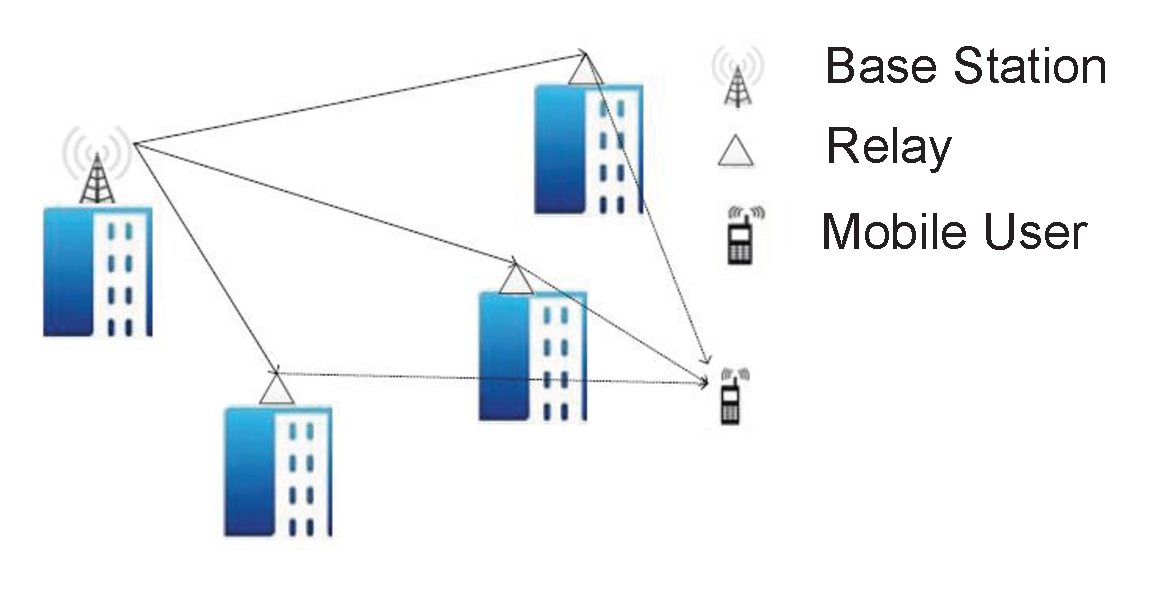
\includegraphics[width=8cm]{buildingversion2.eps}
\caption{Cooperative Communication Example.}
\label{building}
\end{figure}
\par Cooperative communication has been proven to be an efficient way to mitigate fast fading and increase the robustness of data connections \cite{chang2009performance,lee2009performance}. However, cooperative communication can also efficiently maintain the connection whenever the channel condition experiences a sudden deterioration due to shadow fading by switching to different relays. Figure \ref{building} is an example of cooperative communication where relays and BS are placed on the top of buildings. In this case, when the MS moves to the area behind a tall building, with a high probability the signal transmitted from the BS will be obstructed by the building, and consequently the MS will encounter deep shadow fading. The channel  between BS and MS will degrade and data rate will drop suddenly. In the worst case scenario, the connection with the BS may be totally lost. To combat this effect and enhance the signal received by the MS in this case, relays can be deployed on the top of tall buildings to relay the signals from the BS to MS to maintain good channel conditions between the BS and MS.
\par Cooperative communication has been a topic of research for several years. Madan et al. \cite{madan2008energy} studied multi-user spatial diversity in a shadow-fading environment. Other work \cite{emamian2002multi,kasiri2008new,park2011opportunistic}, studied relay selection and cooperative relaying over different fading channels in different systems. Patwari et al. \cite{bletsas2006outage} studied relay placement in realistic deployments and confirmed that Rayleigh fading alone is not an appropriate assumption for evaluating network performance in a real deployment. In \cite{zlatanov2011average, kaltakis2009uplink}, the authors analyzed outage probability and its duration with cooperative relaying. In an 4G-LTE network, which is strongly resilient to multipath fading, shadow fading becomes the most important fading factor \cite{rappaport1996wireless}. Given the presence of relays, the channel variation experienced by an MS in an environment with correlated shadow fading is still an open problem. In this chapter, we analyze this problem in a single cell, and give insights on how relays could mitigate shadow fading. We will derive the critical relay density that can guarantee a certain QoS between the BS and an MS.
\par In most cases, shadow fading is modeled as an independent log-normal distribution \cite{goldsmith2005wireless} with a standard deviation derived from empirical measurements. An independent log-normal shadowing model is used widely when shadow fading cannot be ignored. In the log-normal shadowing model, the path loss $\psi$ is assumed random, with a log-normal distribution given by
\begin{equation}
p(\psi)=\frac{\xi}{\sqrt{2\pi}\sigma_{\psi_{dB}}\psi}exp[-\frac{(10\log_{10}\psi-\mu_{\psi_{dB}})^{2}}{2\sigma_{\psi_{dB}}^{2}}], \psi>0,
\end{equation}
where $\xi=10/\ln10$, $\mu_{\psi_{dB}}$ is the mean of $\psi_{dB}=10\log_{10}\psi$ and $\sigma_{\psi_{dB}}$ is the standard deviation of $\psi_{dB}$.
The distribution of the $dB$ value of $\psi$ is Gaussian with mean $\mu_{\psi_{dB}}$, standard deviation $\sigma_{\psi_{dB}}$ and can therefore also be expressed as:
\begin{equation}
p(\psi_{dB})=\frac{1}{\sqrt{2\pi}\sigma_{\psi_{dB}}}exp[-\frac{(\psi_{dB}-\mu_{\psi_{dB})^2}}{2\sigma_{\psi_{dB}}^2}].
\end{equation}
The above model fails to capture the spatial correlations in shadow fading. Empirical measurements show that shadowing has significant correlations in realistic scenarios that can affect system performance \cite{graziano1978propagation}. Considering the distribution of obstructions and the speed of the MS, a realistic channel propagation model should incorporate correlated shadow fading.  Szyszkowicz et al. \cite{szyszkowicz2010feasibility} presented a review and analysis of the feasibility of different correlated shadowing models.
\par In cooperative communications, relays help the BS to maintain the connection with the MS. Different cooperative schemes can be used by relays. Typically there are two schemes: Amplify-and-Forward (AF), Decode-and-Forward (DF) \cite{nosratinia2004cooperative}. In the AF mode, relays amplify the noisy signal received from the source and forward to the MS. In the DF mode, relays decode the signal received from the BS, then encode it and forward the coded signals to the MS. In this chapter, we assume that DF scheme is used by relays.
\par Given a fixed placement of BS and a fixed moving trajectory for the MS, the efficient placement of relays to maintain the connection between BS and MS and the resulting reduction of the MS's outage probability under correlated shadow fading is the main focus of this chapter. The key contributions of this chapter are summarized below.
\begin{itemize}
\item An analysis of the relationship between correlated shadow fading and correlated outage events.
\item Show how relays help mitigate correlated shadow fading. Correlated outage fields with and without relaying are given and compared.
\item Analyze the performance of three different relay deployment schemes with different relay densities. The performance includes computing the best channel gain and the resulting change in outage probabilities. We also compare the advantages and disadvantages of different relay deployments.
\end{itemize}
The chapter is organized as follows: Section~\ref{sec:Shadow} presents the correlated shadow fading model that is used in this chapter and the resultant correlated outage. Section~\ref{sec:SystemModel} presents the system model with three different relay deployments. Section~\ref{sec:AA} gives theoretical analysis of how relays mitigate shadow fading and reduce outage probability. Section~\ref{sec:Simulation} presents the simulation setup and analyzes the simulation results of different relay deployments. Section~\ref{sec:Conclusions} summarizes the chapter.
\section{Correlated Shadow Fading}
\label{sec:Shadow}
As stated in the introduction, empirical measurements show that there exist different patterns of correlations between the shadowing. The independent log-normal shadow fading model, while very useful for static MS performance analysis, cannot reflect the correlation of shadow fading between different locations. In this section, we will give a brief introduction of shadow fading models, including the model used in this chapter.
\begin{figure}
\centering
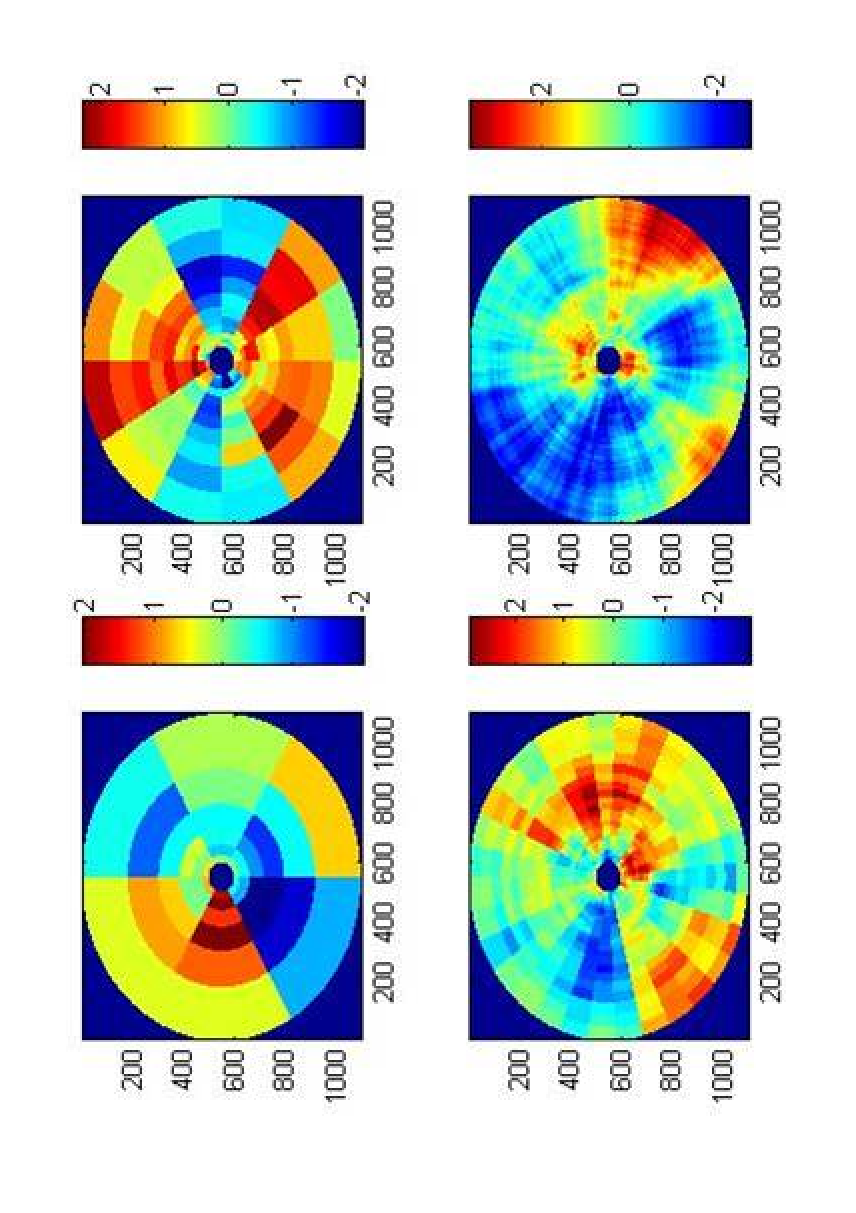
\includegraphics[width=6cm,angle=270]{shadowingfield_V3.eps}
\caption{Correlated Shadowing Fields for Increasing Resolutions (The disk area is the generated correlated shadowing field and the color of the areas refers to the normalized standard deviation which is $S_{i}/\sigma_{s}(\vec{r_{i}})$)}
\label{2:shadowingfield}
\end{figure}
%In most cases, shadow fading is considered as independent log-normal. But from empirical measurements we can see that there exits different correlations between shadow fading factor.
There is no single mathematical model which captures all categories of correlation\cite{szyszkowicz2010feasibility}. In this chapter, we use the correlated shadow fading model which incorporates the angular and distance correlations of shadow fading \cite{szyszkowicz2011interference}. In \cite{szyszkowicz2011interference}, the author states that correlation in shadowing is indispensable for the analysis of interference of large networks and gives a time-efficient fast shadowing fields generation algorithm. The algorithm generates a correlated shadowing field $\vec{S}$, which gives shadow fading factor $\vec{s_{i}}$ for each path $\vec{r_{i}}$ with a correlation matrix
\begin{equation}
\mathbf{K}_{N\times N} = [ \sigma_{s}(\vec{r_{i}})\sigma_{s}(\vec{r_{j}})h(\vec{r_{i}}\vec{r_{j}})],
\label{2:correlationmatrix}
\end{equation}
where $N$ paths interfere with path $\vec{r_{i}}$ and $\mathbf{E}\{S_{i}^{2}|\vec{r_{i}}\}=\sigma_{s}^{2}(\vec{r_{i}})$. This model assumes that in the correlation matrix, $h$ is separable with respect to the angle of arrival
\begin{equation}
\theta = |\angle\vec{r_{i}}-\angle\vec{r_{j}}|\in [0^{\circ},180^{\circ}],
\end{equation}
and the arrival distance ratio
\begin{equation}
R=|10\log_{10}r_{i}/r_{j}|=\frac{10}{\ln 10}|\ln r_{i}-\ln r_{j}|,
\end{equation}
\begin{equation}
h(\vec{r_{i}},\vec{r_{j}})=max\{1-\theta/\theta_{0},0\}\cdot max\{1-R/R_{0},0\}.
\end{equation}
Following the fast shadowing field generation algorithm, we generate shadowing fields with different values of tunable parameters. The shadowing fields are shown in Figure \ref{2:shadowingfield} with increasing resolutions. Four circular correlated shadowing fields are generated.
The shadowing fields are similar to those generated in \cite{szyszkowicz2011interference}.
\subsection{Correlated Outage Field}
\label{2:outagefield}
\begin{figure}
\centering
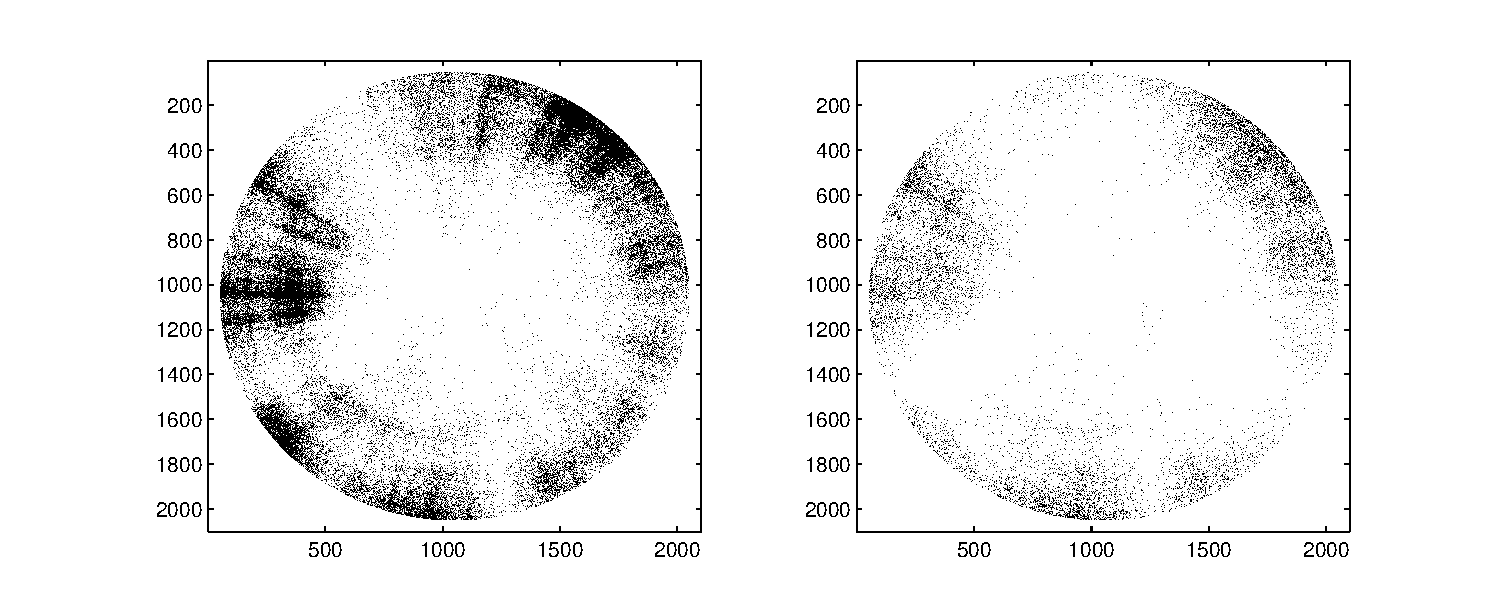
\includegraphics[width=12cm]{outagefield.eps}
\caption{Correlated Outage Fields without (left) and with (right) Relays (Dark areas are outage areas while white areas are non-outage areas)}
\label{2:outagefie}
\end{figure}
Given a correlated shadowing field, the outage events at different locations are also correlated. Here we analyze correlated outage events under correlated shadow fading and later give an example. In the spatial correlation of outage events, without considering Rayleigh fading, path loss is considered as constant at a fixed time point. Based on the correlated shadowing field we can generate a correlated outage field. Let $G$ denotes total channel gain, $PL$ denotes path loss, %$R$ denote the norm of small-scale Rayleigh fading factor,
and $S$ denotes shadow fading factor, we then have:
\begin{equation}
G = PL* S.
\end{equation}
For two different positions, the correlation coefficient of the two total channel gains is of the following form:
\begin{equation}
\rho_{1,2} = \frac{E[G_{1}G_{2}]}{\sqrt{(Var(G_{1})Var(G_{2}))}},
\label{eq1}
\end{equation}
where $G_{1}=PL_{1}*S_{1}$ and $G_{2}=PL_{2}*S_{2}$.
At a fixed time point, temporal correlation is neglected and only spatial correlation is considered, then $PL_{1}$, $PL_{2}$ can be assumed to be constants, which means that $E[PL_{1}] = PL_{1}$, $E[PL_{2}] = PL_{2}$. Based on this assumption, we have
\begin{equation}
E[G_{1}G_{2}] = PL_{1}PL_{2}E[S_{1}S_{2}],
\label{eq2}
\end{equation}
\begin{equation}
Var(G_{1}) = PL_{1}^{2}Var(S_{1}),
\label{eq3}
\end{equation}
\begin{equation}
Var(G_{2}) = PL_{2}^{2}Var(S_{2}).
\label{eq4}
\end{equation}
Based on \eqref{eq2}, \eqref{eq3} and \eqref{eq4}, it is straightforward to rewrite \eqref{eq1} as:
\begin{equation}
\rho_{1,2} = \frac{E[S_{1}S_{2}]}{\sqrt{Var(S_{1})Var(S_{2})}} = \rho_{S_{1},S_{2}}.
\end{equation}
The channel gain has a spatial correlation coefficient as shown above. Based on the result above, a correlated channel gain field can be generated. Given a proper threshold $\gamma$, the correlated outage field can be generated as in Figure \ref{2:outagefie}. On the left, a correlated outage field without relaying is shown while the correlated outage field with relaying (3 relays uniformly placed on a circle near the edge) is given on the right. The black color indicates outage areas. In the next section we will present the methodology that helped us generate the results with relays.

\begin{figure}
\centering
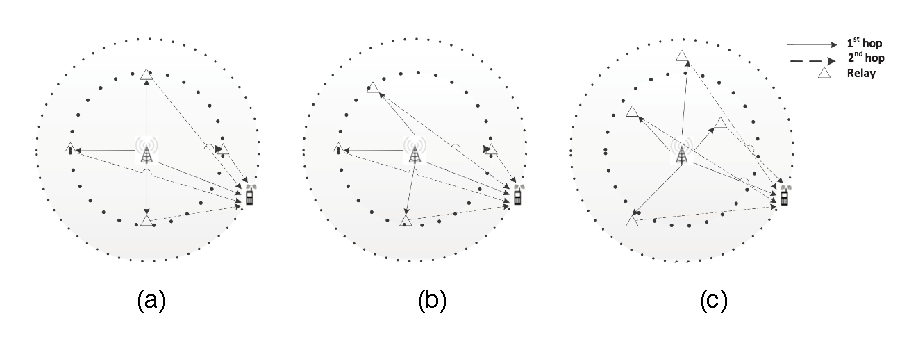
\includegraphics[width=14cm]{abc.eps}
\caption{System Model and Three Different Relay Placements}
\label{threemodels}
\end{figure}
\section{System Model}
\label{sec:SystemModel}
Since most of the key aspects of the problem can be studied in a single cell, we consider a single cell cellular deployment, where the BS is located at the center of the cell.  Figure \ref{threemodels} shows the system model that is used in this chapter. Several relays are placed in the cell and an MS is moving at a particular speed along the circumference at the cell edge. We picked this trajectory since it is the most challenging path given the combination of shadowing and path loss. We consider three relay deployment modes. From left to right in Figure \ref{threemodels}, (a) is the mode where relays are placed uniformly on a circle near the cell edge; (b) is relays that are randomly spaced on a circle near the cell edge; (c) is relays placed randomly in the cell. By varying relay densities in the above three different models we can analyze which combination of relay density and relay placement can meet the required QoS.

\subsection{Cooperative Communication Scheme}
\label{Towhop}
\par In this system, the BS and relays work cooperatively to try to guarantee that the MS has sufficient received power either from the BS or from relays with high probability. There are two main cooperative communication schemes: Amplify-and-Forward, and Decode-and-Forward. In this chapter, we assume that relays use the Decode-and-Forward scheme. The cooperative communication system works in the following manner:
\begin{itemize}
\item First Hop: BS broadcasts signals to both relays and MS. If MS receives and decodes the signals transmitted by the BS successfully, there is no need for relays to repeat the transmission. If not, relays which successfully decode the signals will participate in the second hop retransmission. This mode of operation will require some signaling overhead, which is not addressed in this chapter. Relays which cannot decode the received signal successfully, will not participate in the second hop.
\item Second Hop: Among all relays which participate in the second hop, the one that has the best channel gain between the relay and MS will be chosen (this can be done by centralized control or using information from pilot signals). This relay will encode the signals again and send the coded bits to the MS.
\end{itemize}

\par The received signal in a link $(S\to D)$ between the source and destination is given by:
\begin{equation}
y_{D} = G_{SD}x_{S}+n_{D},
\end{equation}
where $x_{S}$ is the signal transmitted by the source and $y_{D}$ is the signal received by the destination. $n_{D}\sim \mathcal{CN}(0,N_{0})$ is additive white Gaussian noise. $G_{SD}$ is the channel gain from source to destination including path loss and shadow fading. $\text{SNR} \triangleq P*G_{SD}^{2}/N_{0}$, is the end-to-end received signal-to-noise ratio (SNR) and $P$ is the transmitted power. The destination successfully receives the signals if no outage event happens, i.e., $\log_{2}(1+\text{SNR})\ge R$, where $R$ is the required data rate. From the definition of SNR, no outage event happens as long as SNR $> \gamma$, where $\gamma = 2^{R}-1$.
In the first hop, relays that can successfully decode the signals transmitted from the BS is a subset $\mathcal{R}_{n}$ of $N$ relays defined by:
\begin{equation}
\mathcal{R}_{n}\triangleq \{ i: \log_{2}(1+\text{SNR}_{S-i})\ge R\},
\end{equation}
where $\text{SNR}_{S-i}$ is the received signal-to-noise ratio from BS to relay $i$ and $n\in\{0,1,\cdots,2^{N}\}$.
%The channel gain of the source-relay channel is denoted by $X_{i}$ for the $i$th relay where $i\in {1,2,\cdots,N}$, where $N$ is the total number of relays.
In the first hop, the relay can successfully decode the BS signals if $\text{SNR}_{S-i}>\gamma$. The indices of all relays which are able to successfully decode BS signals form a set $\mathcal{R}_{n}$. In the second hop, the selected best relay $j$ is the relay in $\mathcal{R}_{n}$ that has the maximum SNR among all relays in $\mathcal{R}_{n}$, i.e., $j=\arg\max_{i\in \mathcal{R}_{n}}\{\text{SNR}_{i-D}\}$, where $\text{SNR}_{i-D}$ denotes the SNR from the $i$th relay to the destination MS. The BS to MS SNR is denoted by $\text{SNR}_{S-D}$. The SNR is determined by distance related path loss and large-scale correlated shadow fading.

\section{Outage Probability Analysis}
\label{sec:AA}
Due to the variations of the channel gain caused by shadow fading and path loss of the propagation environment, if the  end-to-end  channel capacity is below the transmission rate, an outage occurs and the information packets are lost. The outage probability is an important performance measurement of the communication system. In this section, the expression for outage probability is derived.

\subsection{Outage Probability of the Cooperative Communication System}
\label{outageprobability}
 If an MS cannot directly receive the signal from the BS and none of the relays can decode the BS signal, or if the MS has a bad channel with all relays which successfully decode the BS signal, then an outage event will take place. The probability that an MS cannot receive signals directly from the BS successfully is given below:
\begin{equation}
P_{out_{0}} = P[\text{SNR}_{S-D}<\gamma].
\end{equation}
Under the assumption that an MS cannot successfully receive signals from the BS, the outage event happens in the first hop if no relay can receive the signal from the BS successfully, which means $\mathcal{R}_{0}=\phi$. Based on this assumption we have:
\begin{equation}
P_{out_{1}} = \max_{i = 1,\cdots,N} P[\text{SNR}_{S-i}<\gamma].
\end{equation}
If the outage does not happen in the first hop, then the outage event may happen in the second hop with probability:
\begin{equation}
P_{out_{2}} = \sum_{n=1,\cdots,2^{N}}P[\text{SNR}_{j-D}<\gamma|\mathcal{R}_{n}]P[\mathcal{R}_{n}],
\end{equation}
where $j$ is the index of the relay which has the best channel gain between it and the MS.
So the outage probability of the system is
\begin{equation}
P_{out_{S}} = P_{out_{0}}*(P_{out_{1}}+(1-P_{out_{1}})*P_{out_{2}}).
\end{equation}
The probability density function (pdf) of shadow fading $S$ given $L$ correlated fading branches is
\begin{equation}
\begin{split}
f_{\mathbf{S}}(\mathbf{s}) = &\frac{\lambda^{L}}{\sqrt{2\pi}|\mathbf{K}_{L\times L}|^{1/2}\prod_{i=1}^{L}s_{i}}\\
&\cdot\exp(-\frac{1}{2}(10\log_{10}\mathbf{s}-\boldsymbol{\mu})^{T}\mathbf{K}_{L\times L}^{-1}(10\log_{10}\mathbf{s}-\boldsymbol{\mu})),
\end{split}
\end{equation}
where $\lambda = 10/\ln10$ and $\boldsymbol{\mu}$ is the average shadow fading which is normally $0$. $\mathbf{K}_{L\times L}$ is the correlation matrix which is defined in \eqref{2:correlationmatrix}. Let $\theta_{i} = \frac{10\log_{10}s_{i}-\mu_{i}}{\sqrt{2}\sigma_{i}}$, and doing a change of variables gives us the pdf of $\mathbf{\Theta}$ as follows:
\begin{equation}
f_{\mathbf{\Theta}}(\boldsymbol{\theta}) = \frac{1}{\pi^(L/2)|\mathbf{\Sigma}|^{1/2}}\exp(-\mathbf{\Theta}^{T}\mathbf{\Sigma}^{-1}\mathbf{\Theta}),
\end{equation}
where $\mathbf{\Sigma}$ is the correlation coefficient matrix which is
\begin{equation}
\left[\begin{array}{cccc}
1 & h_{1,2} & \cdots & h_{1,L}\\
\vdots & \ddots & \ddots & \vdots\\
h_{L,1} & h_{L,2} & \cdots & 1\\
\end{array}\right].
\end{equation}
Since SNR $=PL+S-N_{0}$ in dB, SNR$>\gamma$ means $S>\gamma-PL+N_{0}$.
%Without loss of generality, we assume Rayleigh fading has average power $1$. To guarantee $99.9\%$ average successfully transmission, $R_{th}=-7dB$. So shadow fading threshold is $\gamma>\beta-PL+7dB+N_{0}$.
Given $\mathcal{S}_{0}=\phi$, and letting $\gamma_{ai}$ denote the shadow fading threshold for the $i$th relay in the $a$th hop and where $a=0,1,2$, where the $0$th hop is the direct transmission from BS to MS, we then have
\begin{equation}
P_{out_{1}} = \underbrace{\int_{-\infty}^{+\infty}\cdots\int_{-\infty}^{+\infty}}_{i =1,\cdots,N}\prod g_{0}(\gamma_{1i})f(\mathbf{s_{1}})d\mathbf{s_{1}}.
\end{equation}
For $n=1,\cdots,2^{N}$, the outage probability for the second hop is
\begin{equation}
\begin{split}
P_{out_{2}} = \sum_{n=1,\cdots,2^{N}}\underbrace{\int_{-\infty}^{+\infty}\cdots\int_{-\infty}^{+\infty}}_{i=1,\cdots,N}\prod g_{n}(\gamma_{1i}) f(\mathbf{s_{1}})d\mathbf{s_{1}}\\
\cdot\underbrace{\int_{-\infty}^{+\infty}\cdots\int_{-\infty}^{+\infty}}_{i\in \mathcal{R}_{n}}\prod g_{n}(\gamma_{2i})f(\mathbf{s_{2}})d\mathbf{s_{2}},
\end{split}
\end{equation}
where $\mathbf{s_{1}}$ is the correlated shadow fading in the first hop, $\mathbf{s_{2}}$ is the correlated shadow fading in the second hop, $u$ is a step function and
\begin{equation}
g_{n}(\gamma_{ai}) = \{\begin{array}{cc}
               u(\gamma_{ai}) & i\in \mathcal{R}_{n} \\
               1-u(\gamma_{ai}) & i\notin \mathcal{R}_{n}
             \end{array}.
\end{equation}
Due to the random nature of propagation environment, $P_{out_{0}}$ is beyond our control. Therefore, to reduce the outage probability, we need to reduce $P_{out_{1}}$ and $P_{out_{2}}$. Relays at proper positions with sufficient density can reduce the outage probability. Comparing different relay placements and finding the appropriate relay density to guarantee the outage probability requirement is the main issue that we will consider next.

%\par Considering a simple case where we have two relays which are far away from each other (no shadow fading correlation) and all shadow fading factor have the same average $\mu$ and standard deviation $\sigma$, the outage probability is given as:
%\begin{equation}
%P_{out_{0}}=\int_{-\infty}^{\gamma_{00}}f(\mathbf{s})d\mathbf{s}=\Phi(\frac{\gamma_{00}-\mu}{\sigma})
%\end{equation}
%\begin{equation}
%P_{out_{1}}=\int_{-\infty}^{\gamma_{11}}\int_{-\infty}^{\gamma_{12}}f(\mathbf{s1})d\mathbf{s1}=\Phi(\frac{\gamma_{11}-\mu}{\sigma})\Phi(\frac{\gamma_{12}-\mu}{\sigma})
%\end{equation}
%\begin{equation}
%\begin{split}
%P_{out_{2}}=\int_{\gamma_{11}}^{+\infty}\int_{\gamma_{12}}^{+\infty}f(\mathbf{s1})d\mathbf{s1}\int_{-\infty}^{\gamma_{21}}\int_{-\infty}^{\gamma_{22}}f(\mathbf{s2})d\mathbf{s2}\\
%+\int_{\gamma_{11}}^{+\infty}\int_{-\infty}^{\gamma_{12}}f(\mathbf{s1})d\mathbf{s1}\int_{-\infty}^{\gamma_{21}}\int_{-\infty}^{+\infty}f(\mathbf{s2})d\mathbf{s2}\\
%+\int_{-\infty}^{\gamma_{11}}\int_{\gamma_{12}}^{+\infty}f(\mathbf{s1})d\mathbf{s1}\int_{-\infty}^{+\infty}\int_{-\infty}^{\gamma_{22}}f(\mathbf{s2})d\mathbf{s2}\\
%=[1-\Phi(\frac{\gamma_{11}-\mu}{\sigma})][1-\Phi(\frac{\gamma_{12}-\mu}{\sigma})]\Phi(\frac{\gamma_{21}-\mu}{\sigma})\Phi(\frac{\gamma_{22}-\mu}{\sigma})\\
%+[1-\Phi(\frac{\gamma_{11}-\mu}{\sigma})]\Phi(\frac{\gamma_{12}-\mu}{\sigma})\Phi(\frac{\gamma_{21}-\mu}{\sigma})\\
%+[1-\Phi(\frac{\gamma_{12}-\mu}{\sigma})]\Phi(\frac{\gamma_{11}-\mu}{\sigma})\Phi(\frac{\gamma_{22}-\mu}{\sigma})
%\end{split}
%\end{equation}
%where $\Phi$ is the cumulative distribution function (CDF) of the standard normal distribution. For complicated case with correlated shadow fading, numerical analysis can be done and it will give us an idea of how relays can help mitigate correlated shadow fading.
\section{Simulation and Performance Evaluation}
\label{sec:Simulation}
To study which relay placement yields the best system performance i.e., the lowest outage probability for continuous real-time applications that we assume to be running on an MS moving at the cell edge (for the given cooperative communication scheme), we set up simulations and compare performance for different relay placements.
\subsection{Relay Placement}
Different relay placements as shown in Figure \ref{threemodels} are studied and compared in this section.
\begin{itemize}
\item Mode 1: Relays are uniformly spaced on a circle near the cell edge.
    \item Mode 2: Relays are randomly spaced on a circle near the cell edge.
    \item Mode 3: Relays are randomly placed in the cell.
    \end{itemize}
%\subsection{Correlated Shadowing Fields}
%\begin{figure*}
%\centering
%\subfigure[First Hop]{
%\includegraphics[width=4.5cm]{hop1.eps}
%\label{hop1}}
%\hfil
%%\subfigure[Second Hop]{
%%\includegraphics[width = 2.3in,trim= .12in  .73in .62in .4in, clip]{hop1tohop2version2.eps}
%%\caption{TDD half duplex baseline and dull duplex operation.}
%%\label{hop2}
%\subfigure[Second Hop]{
%\includegraphics[width=11cm]{hop1tohop2version33.eps}
%\label{hop2}
%}
%\caption{First Hop and Second Hop Correlated Shadowing Fields. Spatial correlation is demonstrated in the second hop. When MS moves from position A to position B which is one de-correlation distance away from A, a new correlated shadowing field is generated and applied. As we have stated, the cross-correlated shadowing factors associated with links from different relays to the MS can be considered as the auto-correlated shadowing factors associated with the links from MS to different relays.}
%\label{fig4}
%\end{figure*}
%Here, a spatially-correlated shadowing field is generated to reflect the shadow fading factor. Figure \ref{fig4} gives an example of the correlated shadow fading field in the two hop transmission. The shadowing field is coarser than the real one used in the simulation in order to simply and clearly demonstrate the correlated feature of shadow fading. In the first hop, a correlated shadowing field is generated with the BS at the center of the field and with a fixed shadow fading factor corresponding to every relay and every MS position. In the second hop, a correlated shadowing field is generated with the MS at the center of the field. According to \cite{yamamoto2006impact} and \cite{lopez2007resiliency}, auto-correlation and cross-correlation of two interfering paths are very similar and can be studied in the same frame work. Here in our case,
%%the symmetric character between cross-correlation and auto-correlation,
%the cross-correlation of the shadow fading of the links from different relays to MS can be considered as the auto-correlation of the shadow fading of the links from the MS to different relays.
%So only one correlated shadowing field needs to be generated. In both of the two hops, the time-correlation is assumed to be $1$ within $D_{decor}/v$, where $v$ is the speed of the MS and $D_{decor}$ is the de-correlation distance. So an independent correlated shadowing field is generated at every de-correlation distance as shown in Figure \ref{fig4}.

\subsection{Simulation Configuration}
In this chapter, the Okumura-Hata model \cite{saunders2007antennas} is used to estimate the path loss.
%The path loss is
%\begin{align}
%PL_{dB} &= A + B\log_{10}R - E\\
%\text{where } A &= 69.55 + 26.16\log_{10}f - 13.82\log_{10}h_{b}\\
%B &= 44.9 - 6.55\log_{10}h_{b}\\
%E &= 3.2(\log_{10}(11.7554h_{m}))^{2} - 4.97
%\end{align}
%where $R$ is the distance from source to destination[$km$], $h_{m}$ is the destination antenna height above local terrain %height[$m$], $h_{b}$ is the source antenna height above local terrain height[$m$].
%It is assumed that the system undergoes Rayleigh fading, which is small-scale fading in addition to shadow fading.
The values of parameters that are used in the simulation are shown in Table \ref{2:SystemConfig}. In Mode 1 and Mode 2, the radius of the circle where relays are placed (near the edge) is $700m$.
\begin{table}
\centering
\caption{\label{2:SystemConfig}Simulation Configuration Parameters}

\begin{tabular}{|c|c|}

\hline

\multirow{3}{*}{Okumura-Hata Model} & BS Height: $100m$\\
& Relay Height: $10m$\\
& MS Height: $1.5m$\\
\hline
%Rayleigh Fading & Coherence Time: $100ms$\\
%\hline
\multirow{4}{*}{Correlated Shadow Fading} & $R_{0}: 6$\\
& $\theta_{0}: \pi /3$\\
& $d_{min}: 50m$\\
\hline
\multirow{2}{*}{Relay Placements} & Three Modes with Density:\\
& 2,4,6,8,10,12\\
\hline
Cell Size & $R: 1000m$\\
\hline
MS Moving Speed & $v: 10m/s$\\
\hline
Radio Frequency & $f: 900MHz$\\
\hline
BS Transmission Power & $P: 26dbm$\\
\hline
SNR Requirement & $8dB$\\
\hline
\end{tabular}

\end{table}

\subsection{Simulation Results and Analysis}
\begin{figure}
\centering
\includegraphics[width=12cm]{theo_vs_simu_V2.eps}
\caption{Theoretical and Simulated Outage Probability for Mode 1.}
\label{theovssimu}
\end{figure}

\begin{figure}
\centering
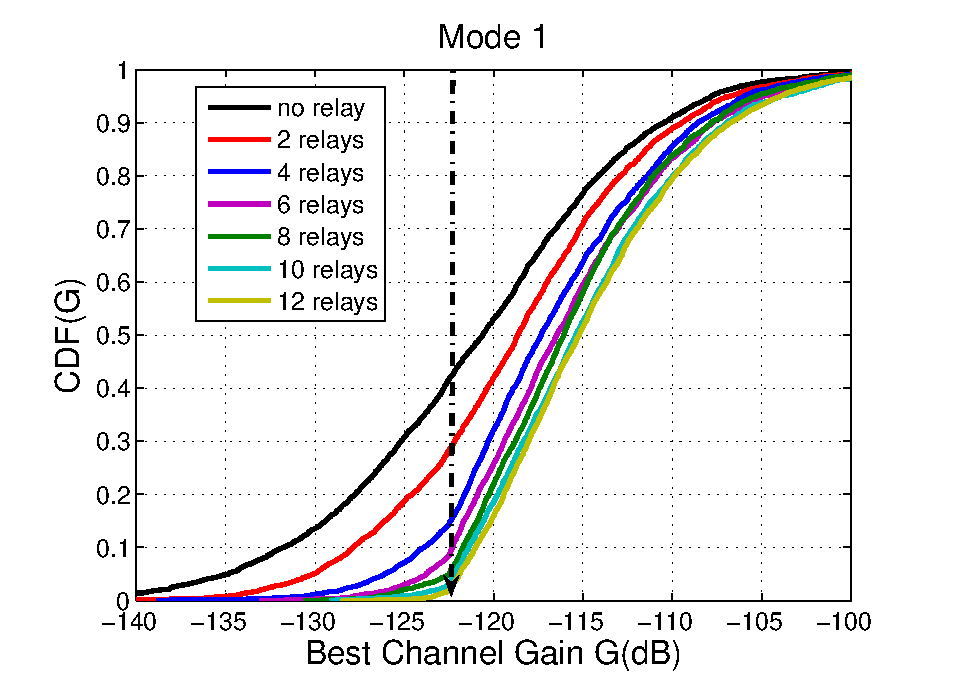
\includegraphics[width=12cm]{Mode1_bestchannelgain_V2.eps}
\caption{Best Channel Condition between MS and BS or Relays of Mode 1 (Dashed arrow demonstrates the channel condition that satisfies the SNR requirement)}
\label{2:Mode1}
\end{figure}
\begin{figure}
\centering
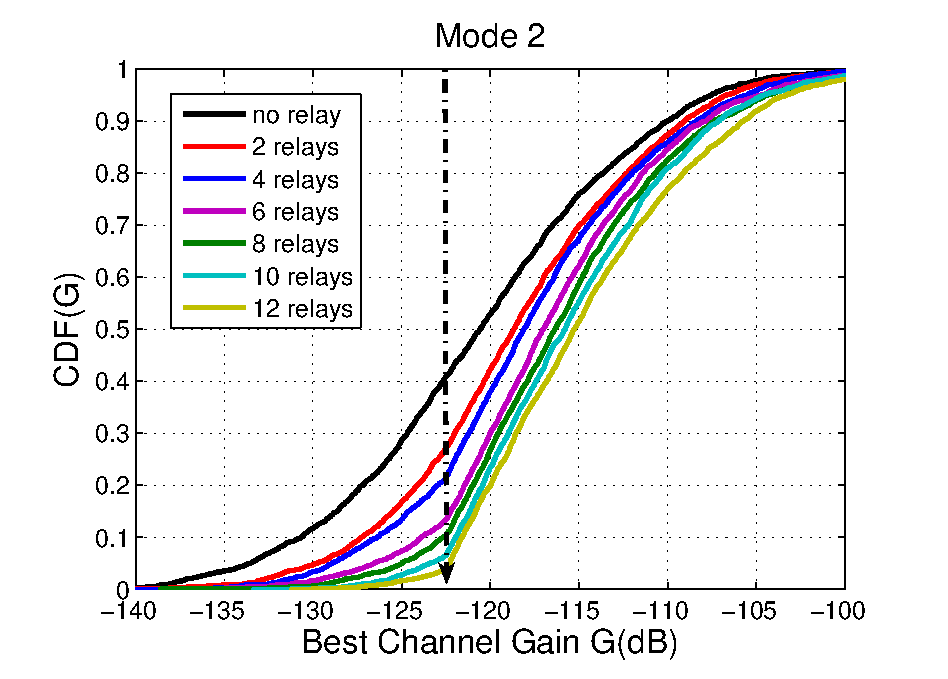
\includegraphics[width=12cm]{Mode2_bestchannelgain_V2.eps}
\caption{Best Channel Condition between MS and BS or Relays of Mode 2 (Dashed arrow demonstrates the channel condition that satisfies the SNR requirement)}
\label{2:Mode2}
\end{figure}
\begin{figure}
\centering
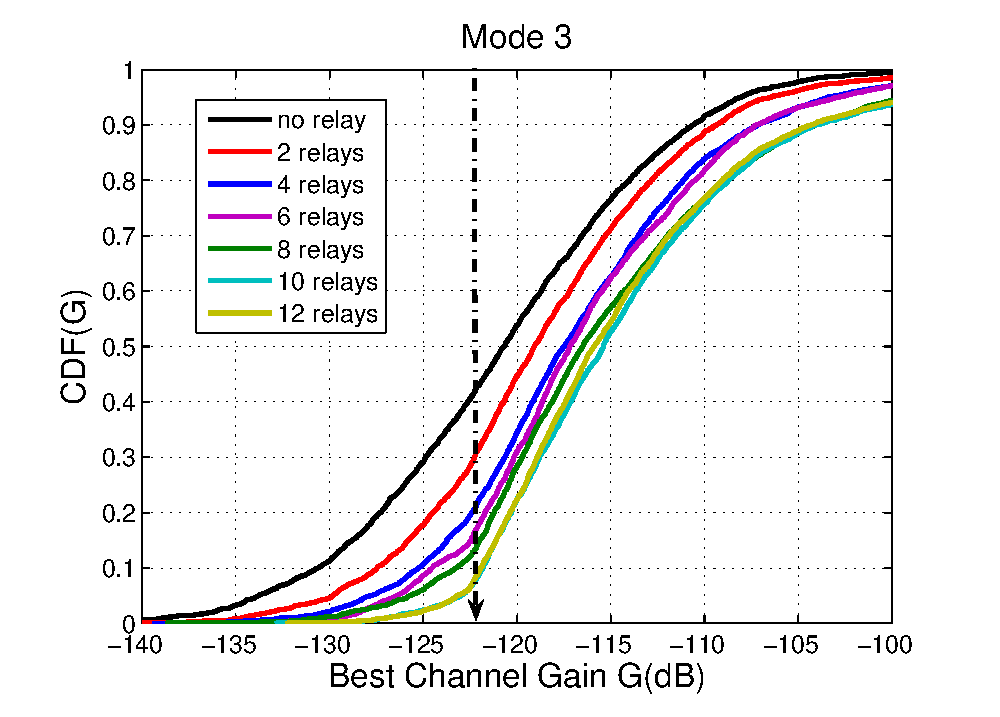
\includegraphics[width=12cm]{Mode3_bestchannelgain_V2.eps}
\caption{Best Channel Condition between MS and BS or Relays of Mode 3 (Dashed arrow demonstrates the channel condition that satisfies the SNR requirement)}
\label{2:Mode3}
\end{figure}
%\caption{Best Channel Condition between MS and BS or Relays (Dashed arrow demonstrates the channel condition that satisfies the SNR requirement.}
%\label{bestchannelgain}
%\end{figure*}
\begin{figure}
\centering
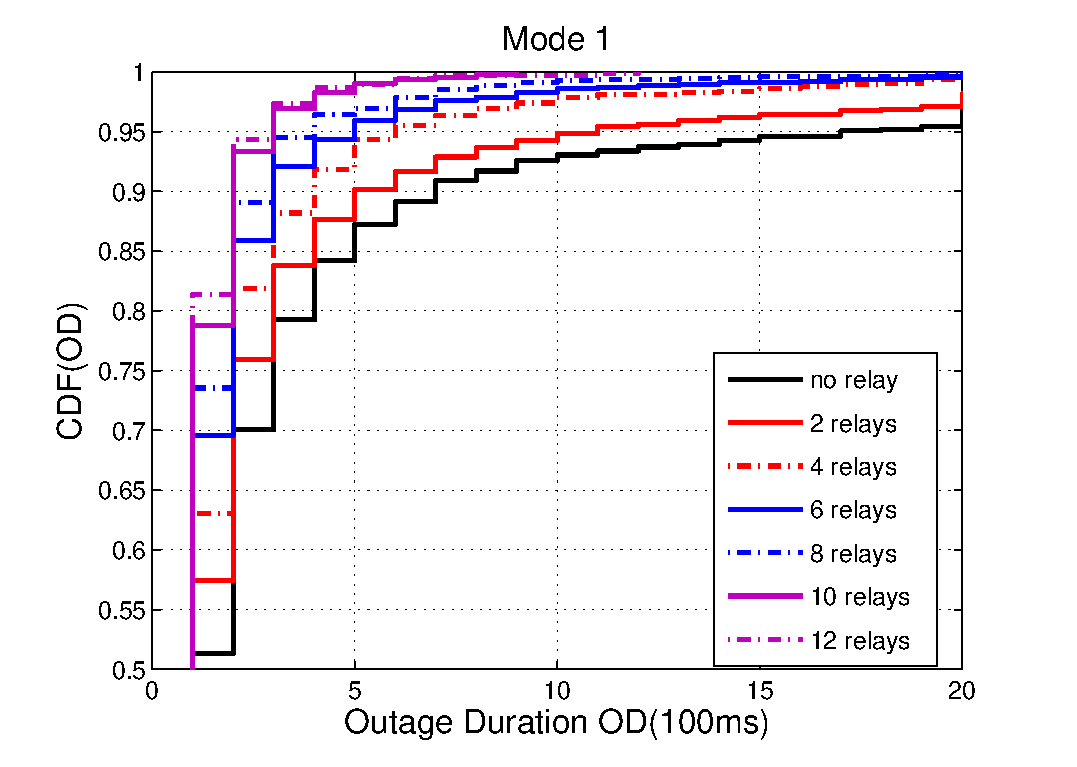
\includegraphics[width=12cm]{OutageDuration_Rayleigh_Mode1_V2.eps}
\caption{Cumulative Distribution Function of Outage Duration of Mode 1 (with Rayleigh fading)}
\label{2:Mode1Out}
\end{figure}
\begin{figure}
\centering
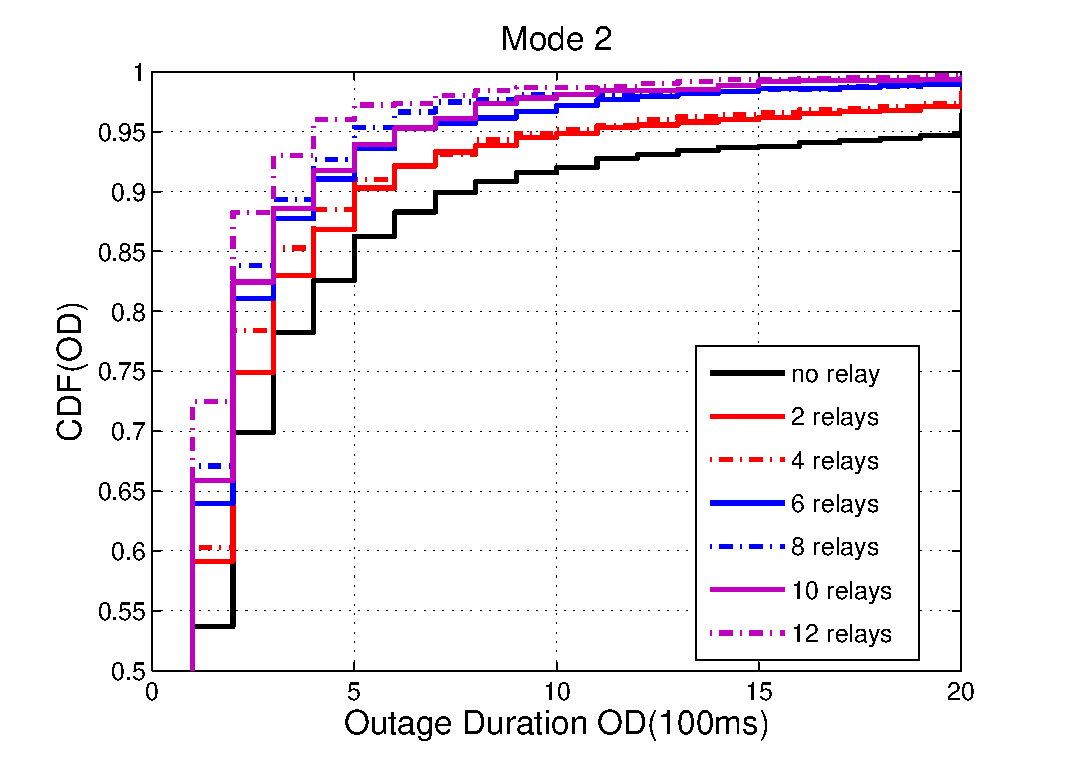
\includegraphics[width=12cm]{OutageDuration_Rayleigh_Mode2_V2.eps}
\caption{Cumulative Distribution Function of Outage Duration of Mode 2 (with Rayleigh fading)}
\label{2:Mode2Out}
\end{figure}
\begin{figure}
\centering
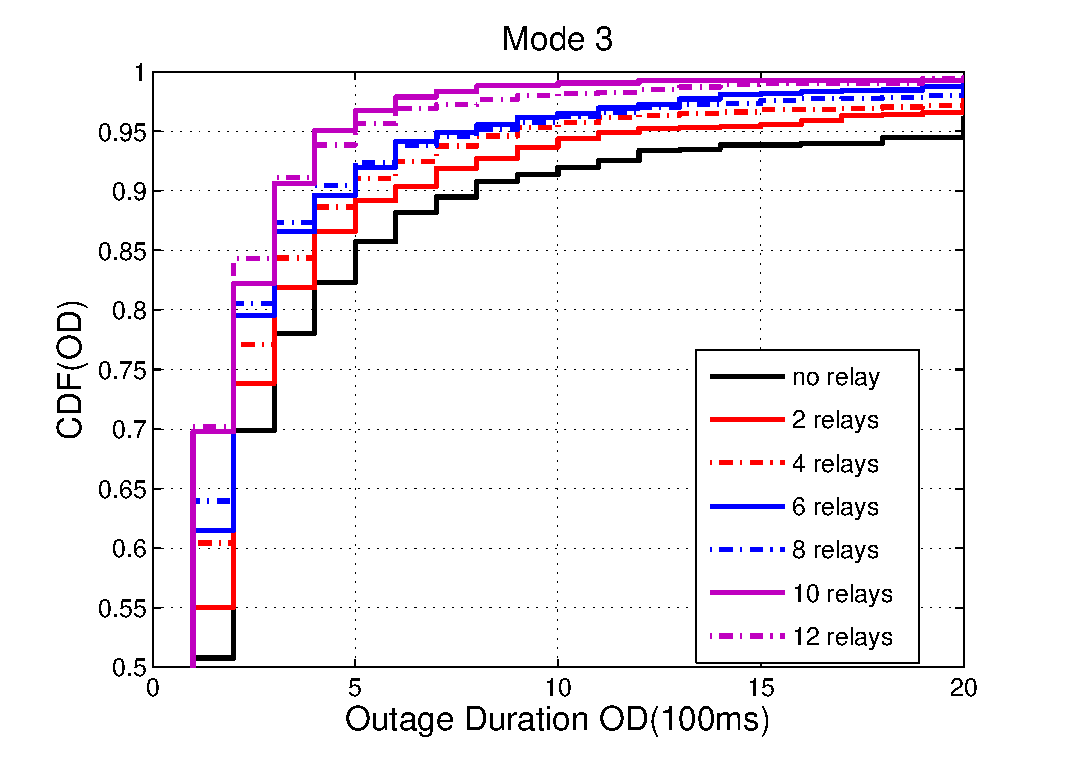
\includegraphics[width=12cm]{OutageDuration_Rayleigh_Mode3_V2.eps}
\caption{Cumulative Distribution Function of Outage Duration of Mode 3 (with Rayleigh fading)}
\label{2:Mode3Out}
\end{figure}
%\begin{figure*}
%\centering
%\subfigure[Mode 1]{
%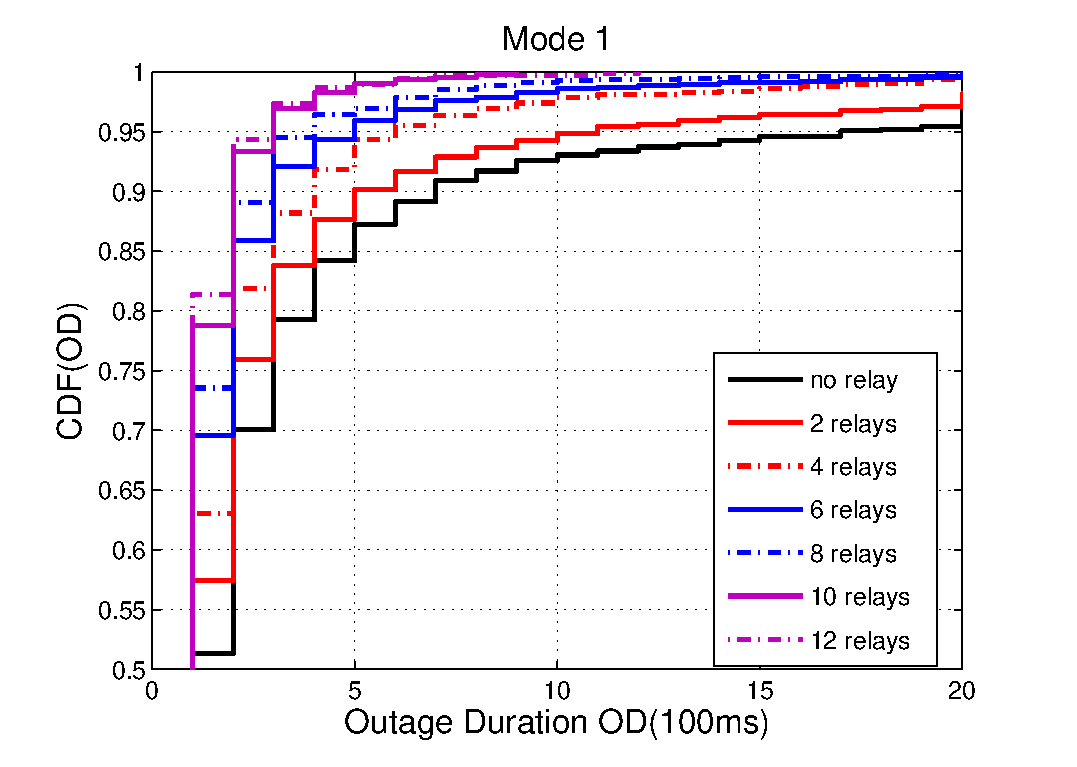
\includegraphics[width=5.5cm]{OutageDuration_Rayleigh_Mode1_V2.eps}
%\label{Mode1}}
%\hfil
%\subfigure[Mode 2]{
%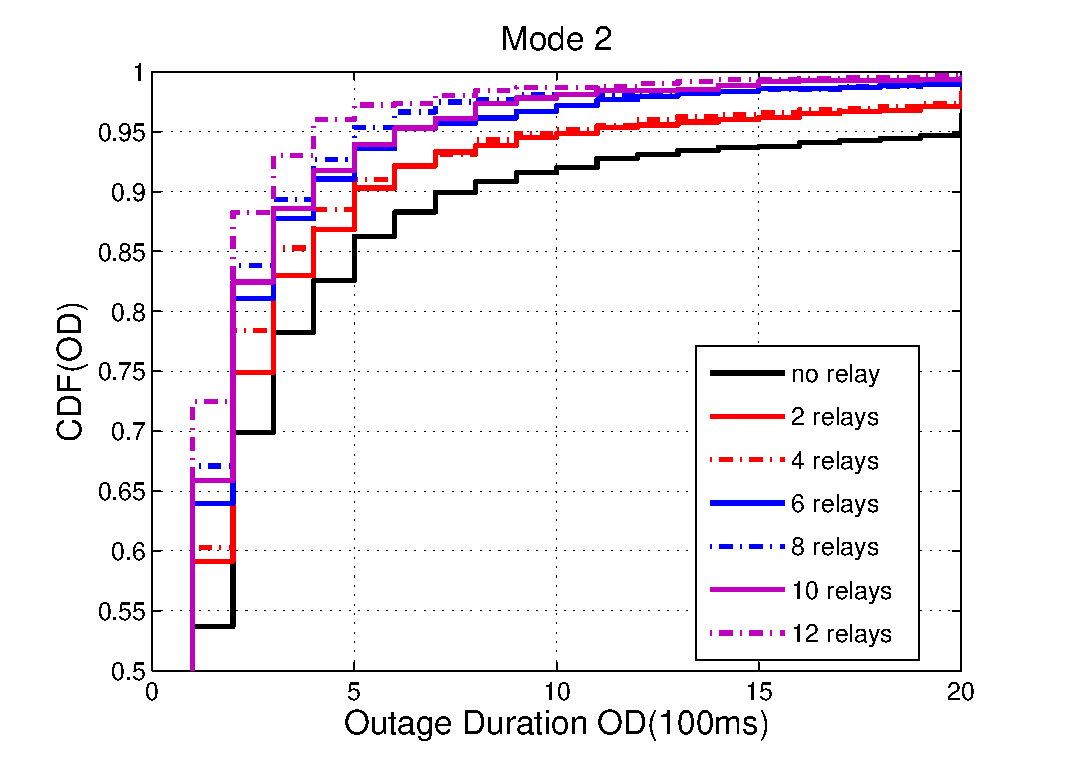
\includegraphics[width=5.5cm]{OutageDuration_Rayleigh_Mode2_V2.eps}
%\label{Mode2}}
%\hfil
%\subfigure[Mode 3]{
%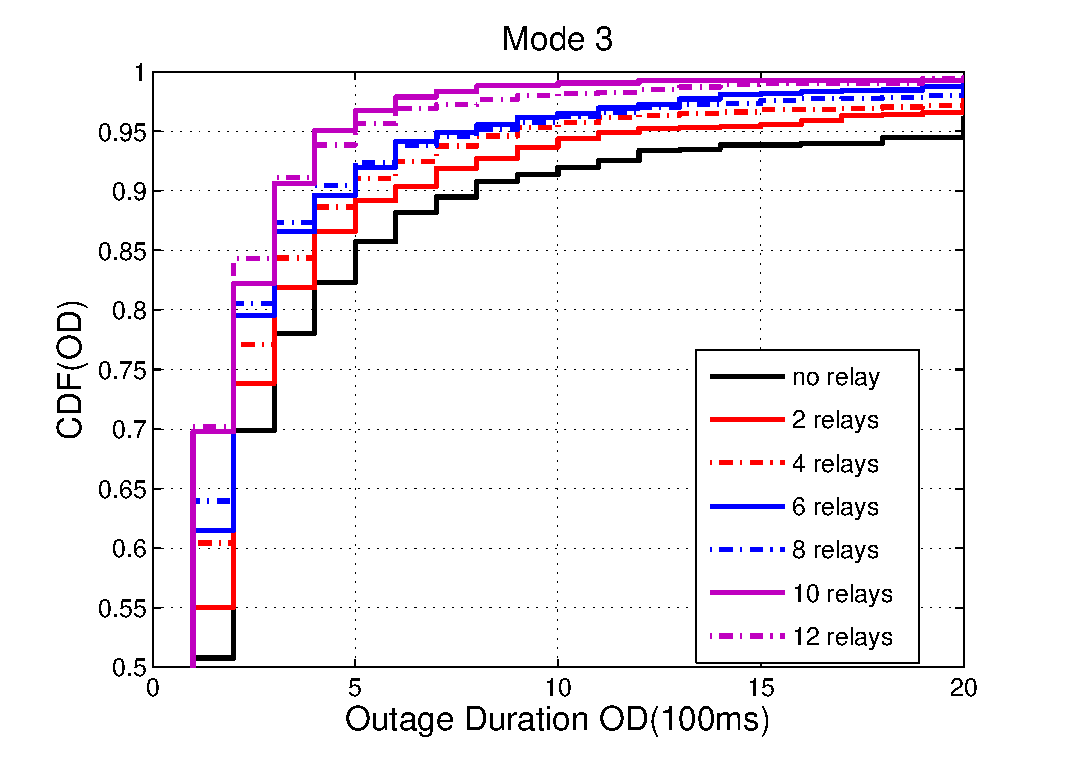
\includegraphics[width=5.5cm]{OutageDuration_Rayleigh_Mode3_V2.eps}
%\label{Mode3}}
%\caption{Cumulative Distribution Function of Outage Duration (with Rayleigh fading)}
%\label{outageperformance}
%\end{figure*}

\par In this section, numerical analysis and simulation results are presented. The best channel condition that the user can get from either BS or relay is simulated to demonstrate the improvement of the received signal strength at the MS. The outage probabilities and durations are shown to indicate the potential user experience improvement when using a real-time application.
\par First, numerical analysis and simulation results of outage probabilities in Mode 1 is shown in Figure \ref{theovssimu}. The numerical analysis has high computational complexity and is difficult to apply to outage duration analysis. Therefore a simulation is necessary to study the system. Considering the computational complexity, to show that our simulation is validated by analysis, partial comparison between numerical analysis and simulation results is shown in Figure \ref{theovssimu}, which indicates that our simulation code is correct and can be used to study the system.
\par Second, we simulate the distribution of the best channel gain for the channel between the MS and BS or relays. Figure \ref{2:Mode1}, \ref{2:Mode2}  and \ref{2:Mode3} plot the distribution of the user channel gain of the three different relay deployment modes and 6 different relay densities. As shown in the figure, the intersection of the dashed arrow and the cumulative distribution function (cdf) plots indicates that as relay density increases, the percentage of outages reduces. The dashed arrow points to $122.5dB$ which is the lowest channel gain to guarantee the SNR to be above $8dB$, in which case 16-QAM with $1/2$ code rate will still work. Considering the power constraints, the complexity and cost of placing relays and received SNR requirements, finding a proper relay density is very important. Beyond a certain relay density, increasing the relay density will not give significant additional performance improvement. In all modes, it is shown that relays can mitigate the shadow fading efficiently. For example, in the Mode 1 case, $10$ relays can improve the performance by reducing the probability of outage by $40\%$ compared to the no relay case. To compare the results across the three different modes, we take the 10 relay case as an example. For this case, Mode 1 has an outage probability $3\%$ less than Mode 2 and $10\%$ less than Mode 3. In addition, we compare the three different modes from the outage frequency point of view. Outage frequency is defined as
\begin{equation}
f_{outage}=\frac{\text{Total Number of Outage Points}}{\text{Total Number of Simulation Points}}.
\end{equation}
\begin{figure}
\centering
\includegraphics[width=12cm]{outagefrequency_V2.eps}
\caption{Outage Frequency of Three Modes with Different Relay Densities}
\label{2:outagefrequency}
\end{figure}
Figure \ref{2:outagefrequency} shows the result of outage frequency of the three different modes and different relay densities. From this result, we can see that Mode 1 performs better than Mode 2 and Mode 3. This is due to the randomness of the relay deployment, which works against outage prevention for this model. In some cases Mode 3 performs better than Mode 2. This occurs when most of the relays in Mode 2 are placed in deep shadow areas and are therefore ineffective.. The ideal relay deployment scheme would place relays at the edge of a deep fading area so that relays can successfully receive signals from the BS. On the average, random placement (Mode 3) is the worst choice among the three cases in our simulation.
\par For real-time applications, outage duration and outage frequency are both very important factors from the user experience point of view. Long outage duration and high outage frequency will lead to poor delay performance or even loss of packets. Figure \ref{2:outagefrequency} indicates that higher relay density will result in lower outage frequency. Next we investigate the outage duration experienced by the MS with different relay deployments. Outage duration performance is given in Figure \ref{2:Mode1Out}, \ref{2:Mode2Out} and \ref{2:Mode3Out}, which shows the cumulative distribution functions for outage durations for all three different modes. Here, we just show the distribution of outage duration from $100ms$ to $2s$ ($100ms$ is the smallest simulation time period). Under the SNR requirement given as $8dB$, it is shown that as the relay density increases, the probability of long outage duration decreases quickly. In Mode 1, with 4 relays, the probability of outage duration longer than $400ms$ is less than $10\%$. In Mode 2 and Mode 3, to achieve this, 6 and 8 relays are needed, respectively. For real-time video conferencing, the largest tolerable delay is around $200ms$. Our results indicate that in Mode 1 we do not need more than 6 relays to guarantee the probability of outage duration larger than $200ms$ to be less than $15\%$. In Mode 2 and Mode 3 more than 12 relays are needed to achieve this objective. Since we put the SNR requirement as $8dB$, which guarantees a small bit error rate (BER) of 16-QAM, the relay density needs to be high. If we reduce the SNR requirement and change the modulation, it is possible that the probability of outage duration longer than $200ms$ will become smaller or even close to 0. If there is no relay in the cell and an MS enters into a deep fading area, then due to correlated shadow fading, this outage duration will last for a long time. The longest outage duration in our simulation is $10s$ with no relay. From Figure \ref{2:Mode1Out}, \ref{2:Mode2Out} and \ref{2:Mode3Out} we can observe that the probability of an outage duration greater than $2s$ is approximately $5\%$ without relaying. Comparing the no relay case with the 6 relays case in Mode 1, it is shown that relays efficiently reduce the lengthy outages which are caused by deep shadow fading, with the probability of outage duration greater than $2s$ reduced to less than $1\%$. All these results indicate that relays can mitigate the deleterious effects of correlated shadow fading efficiently.

\section{Chapter Summary}
\label{sec:Conclusions}
In this chapter, we investigate the correlated shadow fading problem in a single cell cellular network and shows that it could lead to correlated outage and long outage durations. A correlated outage field is presented in this chapter. To mitigate shadow fading, relays can be deployed. The performance of three different relay deployments with different relay densities are studied. Theoretical analysis and simulations of outage performance are given to compare between different relay placement scenarios. Through these simulation, we showed that uniformly spaced relays perform better than the randomly spaced, due to the randomness of relay deployment. In following chapters, we will consider different shadow fading correlation model and extend the research to a multi-cell system. 





